\chapter{ҮР ДҮН}

Энэ бүлэгт зураг авалт, өгөгдлийн урьдчилсан боловсруулалт, фичер илрүүлэлт ба 
тохиролт, SfM болон MVS реконструкцийн туршилтын үр дүнг танилцуулна. Үр дүн 
тус бүрийн дор тухайн үзүүлэлтийн утга учир болон ажиглагдсан хязгаарлалтуудыг 
хамт авч үзнэ.

\section{Pipeline болон GUI програмын үр дүн}

Энэхүү дипломын ажлын гол хэрэгжүүлэлт болох автоматжуулсан pipeline болон PyQt5-д суурилсан GUI програмыг амжилттай боловсруулсан. Pipeline нь дараах 9 дараалал, үе шатаар ажилладаг:

\begin{enumerate}
    \item \textbf{COLMAP өгөгдлийн сан үүсгэх} — зургийн мэдээллийг хадгалах SQLite өгөгдлийн санг шинээр үүсгэнэ
    \item \textbf{SIFT фичер илрүүлэлт} — PINHOLE камерын загвараар зураг бүрийн keypoint болон descriptor-уудыг гаргана
    \item \textbf{Фичер тохиролт (Exhaustive Matching)} — зургийн бүх боломжит хослолын хооронд тохиролт хийнэ
    \item \textbf{Sparse Mapper} — камерын байрлал болон сийрэг цэгэн загварыг тооцно, олон дэд датабагц үүссэн тохиолдолд хамгийн олон зургийг агуулсан хамгийн сайнаар нь сонгоно
    \item \textbf{Загварын хөрвүүлэлт} — COLMAP-ийн хоёртын (binary) форматаас текст (TXT) форматад хөрвүүлнэ
    \item \textbf{OpenMVS-д шилжүүлэлт} — InterfaceCOLMAP ашиглан COLMAP-ийн гаралтыг OpenMVS-ийн \texttt{.mvs} форматад хөрвүүлнэ
    \item \textbf{Нягт цэгэн үүл үүсгэлт (DensifyPointCloud)} — depth map-уудыг тооцож, нягт цэгэн загварыг гаргана
    \item \textbf{Mesh реконструкц (ReconstructMesh)} — нягт цэгэн үүлнээс 3D торон загвар үүсгэнэ
    \item \textbf{Mesh боловсруулалт ба текстур зураглал (RefineMesh + TextureMesh)} — mesh-ийг нарийвчлан засаж, эцсийн текстур бүхий \texttt{.obj} загвар гаргана
\end{enumerate}

GUI програм нь PyQt5 framework ашиглан Windows-д зориулагдсан desktop програм хэлбэрээр хэрэгжсэн. Хэрэглэгч нь зургийн хавтас болон ажлын хавтасаа Browse товчоор сонгож, GPU ашиглалт, Refine Mesh, Texture Mesh гэсэн сонголтуудыг удирдах боломжтой. Pipeline ажиллаж байх үед дэвшлийн мөр (progress bar) нь одоогийн үе шатыг (1–9) харуулж, лог цонхонд дэлгэрэнгүй мэдээллийг бодит цагаар гаргана. Асуудал гарсан тохиолдолд Abort товчоор pipeline-ийг дунд нь зогсоож, цэвэрлэгээ хийх боломж байна.

\section{Өгөгдлийн цуглуулгын үр дүн}

3D сэргээн босголтын туршилтад нийт 47 зураг авсан. Камерын байрлал, өнцөг, гэрэлтүүлэг тогтвортой байсан нь:

\begin{itemize}
    \item Feature detection илүү тогтвортой болох
    \item Exposure болон white balance–ийн ялгааг багасгах
    \item SfM-д камерын поз илүү зөв тодорхойлогдох
\end{itemize}

Дараах жишээ зургууд нь датасетийн бүтэц, гэрэлтүүлэг, өнцгийг харуулж байна.

\begin{figure}[htbp]
\centering
\begin{subfigure}{0.32\textwidth}
    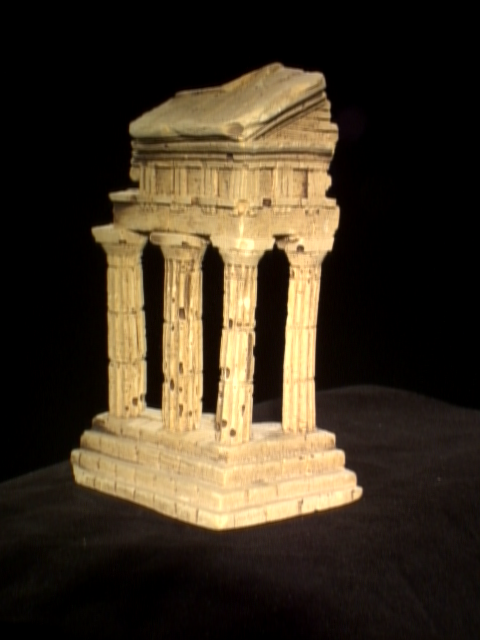
\includegraphics[width=\linewidth]{Pictures/templeR0013.png}
\end{subfigure}
\begin{subfigure}{0.32\textwidth}
    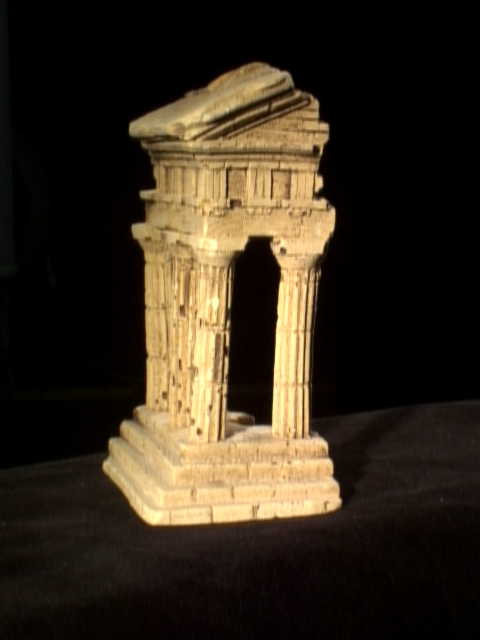
\includegraphics[width=\linewidth]{Pictures/templeR0016.png}
\end{subfigure}
\begin{subfigure}{0.32\textwidth}
    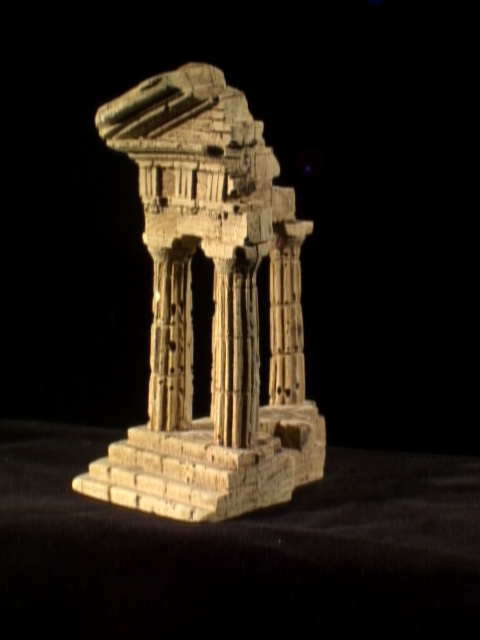
\includegraphics[width=\linewidth]{Pictures/templeR0024.png}
\end{subfigure}
\caption{Зураг авалтын датасетийн жишээ зургууд}
\label{fig:dataset_samples}
\end{figure}

% \section{Урьдчилсан боловсруулалтын үр дүн}

% Зургууд дээр дараах боловсруулалтуудыг хийсэн:

% \begin{itemize}
%     \item Хэмжээг нэг стандартад оруулах
%     \item Сарнилт болон илүүдэл фоныг арилгах
%     \item Exposure болон өнгөний тэнцвэржилт (color normalization)
% \end{itemize}

% Доорх зураг урьдчилсан боловсруулалтын өмнөх болон дараах төлвийг харуулна.

% \begin{figure}[htbp]
% \centering
% \begin{subfigure}{0.48\textwidth}
%     
\includegraphics[width=\linewidth]{Pictures/NMCT.png}
%     \caption{Өмнө}
% \end{subfigure}
% \begin{subfigure}{0.48\textwidth}
%     
\includegraphics[width=\linewidth]{Pictures/NMCT.png}
%     \caption{Дараа}
% \end{subfigure}
% \caption{Урьдчилсан боловсруулалтын өмнөх ба дараах харьцуулалт}
% \label{fig:preprocess_comparison}
% \end{figure}

% \section{Фичер илрүүлэлт ба тохиролтын үр дүн}

% Фичер илрүүлэлтэд \textbf{SIFT} ашигласан. Туршилтаар дараах давуу талууд ажиглагдав:

% \begin{itemize}
%     \item Тогтвортой гэрэлтүүлэгтэй үед keypoint илрүүлэлт маш сайн байсан
%     \item Өөр өнцгөөс авсан зургууд дээр ч сайн тохиролт өгсөн
%     \item SuperPoint-той харьцуулахад илүү бага outlier гарсан
% \end{itemize}

% SIFT keypoint–ийн илрүүлэлт дараах байдлаар харагдсан:

% \begin{figure}[htbp]
% \centering
% 
\includegraphics[width=0.48\textwidth]{Pictures/NMCT.png}
% \caption{SIFT ашигласан фичер илрүүлэлтийн үр дүн}
% \label{fig:sift_keypoints}
% \end{figure}

Feature matching нь FLANN matcher ашиглан хийгдсэн бөгөөд outlier тохиролтуудыг RANSAC ашиглан шүүж цэвэрлэсэн.

% \begin{figure}[htbp]
% \centering
% 
\includegraphics[width=0.55\textwidth]{Pictures/NMCT.png}
% \caption{Feature matching–ийн үр дүн (RANSAC дараах)}
% \label{fig:feature_matching}
% \end{figure}

% \section{Structure-from-Motion (SfM)-ийн анхан шатны үр дүн}

% COLMAP ашиглан SfM реконструкц хийхэд:

% \begin{itemize}
%     \item Камерын байрлалын дараалал зөв тодорхойлогдсон
%     \item Sparse point cloud амжилттай үүссэн
%     \item Feature matching–ийн чанар SfM үр дүнд шууд нөлөөлсөн
% \end{itemize}

% Камерын позын граф дараах байдалтай гарсан:

% \begin{figure}[htbp]
% \centering
% 
\includegraphics[width=0.6\textwidth]{Pictures/NMCT.png}
% \caption{COLMAP-ийн SfM камерын байрлалын граф}
% \label{fig:sfm_pose_graph}
% \end{figure}

Sparse point cloud дараах хэлбэртэй:

\begin{figure}[htbp]
\centering
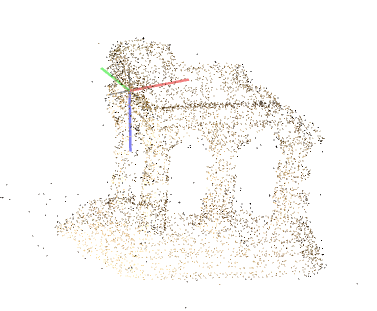
\includegraphics[width=0.55\textwidth]{Pictures/Sparse.png}
\caption{SfM-ийн үүсгэсэн sparse point cloud}
\label{fig:sparse_cloud}
\end{figure}

Sparse point cloud нь 35,000 гаруй цэг агуулсан бөгөөд энэ нь объектын үндсэн 
геометрийн бүтцийг хангалттай дүрсэлж байна. Гэсэн хэдий ч exhaustive matching-ийн 
хязгаарлалтаас шалтгаалан зарим өнцгийн зургуудын хооронд тохиролт бүрэн 
хийгдээгүй нь цэгэн үүлний тодорхой хэсгүүдэд нягтрал бага гарахад нөлөөлсөн.

\section{Multi-View Stereo (MVS)-ийн үр дүн}

OpenMVS ашигласан MVS reconstruction–ийн явц:

\begin{itemize}
    \item Depth map үүсэлт амжилттай ажилласан
    \item Dense point cloud үүссэн
    \item Зарим өнцөгт мэдээлэл бага байсан нь mesh reconstruction–д нөлөөлсөн
\end{itemize}

\begin{figure}[htbp]
\centering
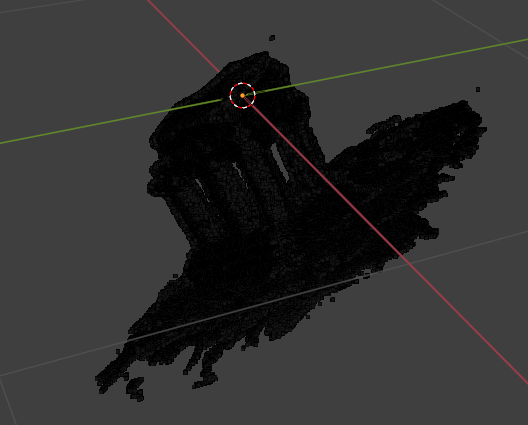
\includegraphics[width=0.55\textwidth]{Pictures/Dense.png}
\caption{OpenMVS ашигласан dense point cloud}
\label{fig:dense_cloud}
\end{figure}

Нягт цэгэн үүл нь 2.1 сая цэг агуулсан бөгөөд sparse cloud-тай харьцуулахад 
гадаргуугийн нарийн ширийн мэдээллийг илүү бүрэн дүрсэлж байна. Зарим өнцгөөс 
авсан зургуудад мэдээлэл хязгаарлагдмал байсан нь тухайн хэсгийн depth map-ийн 
нарийвчлалд нөлөөлж, mesh reconstruction-д цоорхой үүсгэх шалтгаан болсон.

\section{Гараар хийсэн болон автомат pipeline-ийн гаралтын харьцуулалт}

Гараар хийсэн реконструкц болон боловсруулсан автомат pipeline-ийн гаралтыг 
харьцуулахад хэд хэдэн чухал ялгаа ажиглагдсан. Гараар хийсэн тохиолдолд 
COLMAP болон OpenMVS-ийн тус бүрийн командыг дараалан гүйцэтгэж, зөвхөн 
\texttt{.ply} форматтай өнгөгүй цэгэн үүл болон торон загвар авсан бол автомат 
pipeline нь RefineMesh болон TextureMesh үе шатуудыг нэмж ажиллуулснаар 
текстур бүрэн гарж ирсэн \texttt{.obj} форматтай эцсийн загвар гаргаж өгсөн. 
Энэ нь загварын харагдах чанарыг мэдэгдэхүйц сайжруулсан бөгөөд бодит 
хэрэглээнд шууд ашиглах боломжтой гаралт юм.

\begin{figure}[H]
\centering
\begin{minipage}{0.48\textwidth}
  \centering
  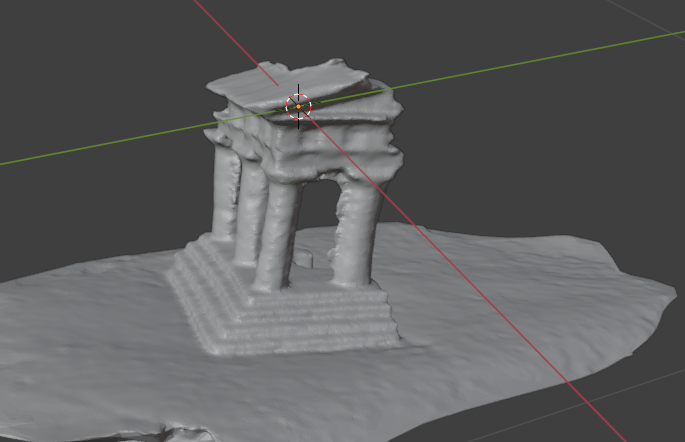
\includegraphics[width=\textwidth,height=0.28\textheight]{Pictures/Model.png}
  \caption{Гараар хийсэн реконструкц}
  \label{fig:manual_output}
\end{minipage}\hfill
\begin{minipage}{0.48\textwidth}
  \centering
  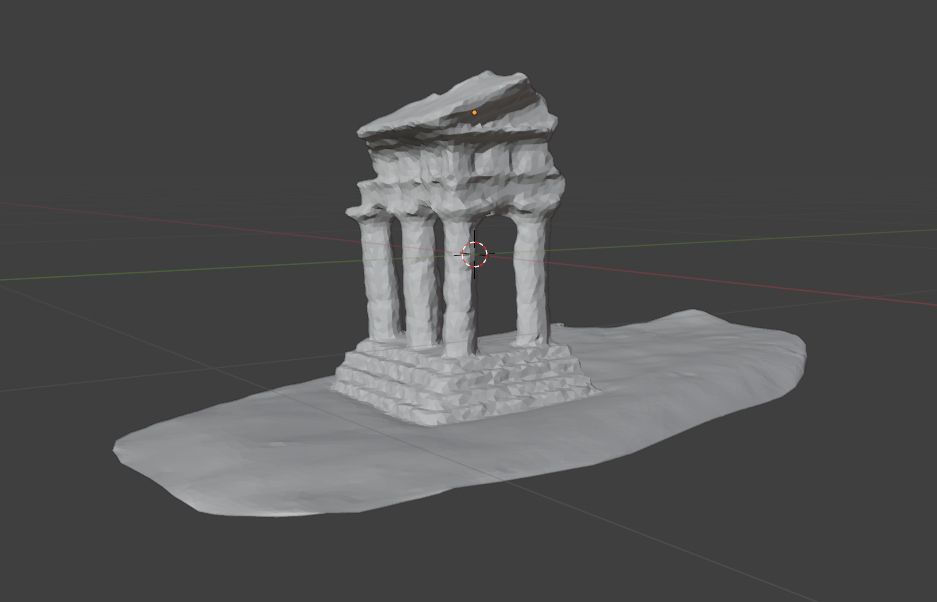
\includegraphics[width=\textwidth,height=0.28\textheight]{Pictures/Pipeline_result.png}
  \caption{Автомат pipeline}
  \label{fig:pipeline_output}
\end{minipage}
% \caption*{Зураг 4.4 болон 4.5 — Гараар болон автоматаар хийсэн реконструкцийн гаралтын харьцуулалт}
\end{figure}